\documentclass[12pt]{article}
\usepackage{fancyhdr}
\pagestyle{fancy}
\fancyhf{}
\fancyhead[R]{\thepage}
\usepackage[margin=1in]{geometry}
\usepackage{graphicx}
\usepackage[hang,flushmargin,ragged]{footmisc}
\renewcommand{\footnotelayout}{\fontsize{12}{8}\selectfont\raggedright}
\setlength{\footnotemargin}{1em}
\usepackage{lipsum,setspace}
\usepackage{amsmath,amsthm,amssymb}
\usepackage{graphicx}
\usepackage{booktabs,float}
\usepackage{flafter}
\usepackage{siunitx}
\renewcommand{\arraystretch}{1.5}
\usepackage[tableposition=top]{caption}
\usepackage[flushleft]{threeparttable}
\usepackage{tablefootnote}
\usepackage{authblk}
\usepackage{parskip}
\usepackage[usenames, dvipsnames]{color}
\usepackage[final]{pdfpages}
\usepackage{placeins}
\usepackage{color}   %May be necessary if you want to color links
\usepackage{hyperref}
\hypersetup{
    colorlinks=true, 
    linktoc=all, 
    linkcolor=blue, 
}
\usepackage{setspace} 
\doublespacing
\usepackage{tocloft}
\renewcommand{\cftpartleader}{\cftdotfill{\cftdotsep}} % for parts
\renewcommand{\cftchapleader}{\cftdotfill{\cftdotsep}} % for chapters
\renewcommand{\cftsecleader}{\cftdotfill{\cftdotsep}} % for sections, if you really want! (It is default in report and book class (So you may not need it).

\setlength\parindent{24pt}
\title{Replication: Small Aggregates, Big Manipulation: Vote Buying Enforcement and Collective Monitoring}
\author{Haseeb Bajwa, Rithika Kumar, John Matthews}


\begin{document}

\maketitle
\tableofcontents
\section{Introduction}

Rueda (2016) tackles an important topic that concerns vote buying incentives in Latin America. Specifically, Rueda looks at the incentives and conditions under which parties ensure compliance of voters. This replication exercise is divided into two sections. In the first section we present our replication of Rueda (2016). Following that we present our extensions to the paper which are focused on Table 2 and Table 3 in the article. These tables contain the most important findings of the paper. 

In the first part of the extension we present the results (from both tables) separately for national and state level elections. Next we drop outlier values of observer reports of vote buying in order to ensure that the results are not being overestimated due to these observations. Next, we identify the five most populous \textit{departamentos} in Colombia and re-run the analysis on this sub-sample of observations.

\section{Replication: Rueda (2016)}

\subsection{Descriptive Statistics}
 
Below are the results of the summary statistics of the monitor's and citizen's reports of vote buying. These two variables are the key dependent variables considered in Table 2 and 3. This table also includes the distribution of registered voters and population over 20 years of age. 
\FloatBarrier
\begin{table}[]
    \caption*{Summary Statistics}
    \centering
\scalebox{0.80}{
\begin{tabular}{l*{1}{ccccc}}
\hline
                     Variable & Obs & Mean & Std.Dev & Min & Max\\
\hline
Citizens Reports&4352&0.222&0.9796&0&29\\
Monitor's Reports&1069&0.280&1.409&0&27\\
\hline
Registered Voters &4352&356.1835 & 57.43899& 171.8095&592.5172\\
Pop + 20 years &4352&318.3925 & 84.05138& 108.0455&1110.75\\

\hline

\end{tabular}
}
\end{table}
\FloatBarrier
\subsection{Results: Table 2}

Our replication covers tables 2 and 3 in the paper, which constitute the main results of the research.  
In Table 2, Rueda lays out the results of regressions of reported incidents of vote buying by  (1) the natural log of registered voters per polling station (2 and 3) the natural log of population above 20 per polling station. Regression (3) introduces a series of controls: measures of economic development, whether armed non-state actors are present, whether elections are competitive, and the size of the voting population. 


\FloatBarrier
\begin{table}[]
    \caption*{Simple Replication of Table 2}
    \centering
\scalebox{0.80}{
\begin{tabular}{l*{1}{ccc}}
\hline
                    Dependent Variable &\multicolumn{3}{c}{Citizens' Vote Buying Reports}\\
                   Size Measure &\multicolumn{}{c}{ln(Registered / Stations)}&\multicolumn{2}{c}{ln(Pop. age \geq 20 / Stations)}\\
                    &(1)&(2)&(3)\\
\hline
Polling Place Size&-1.929&-1.544&-1.1158\\
                    &(0.3633)&(0.2321)&(0.2509)\\

Armed Group &&&-0.32402\\
                  &&&(0.1225)\\

Electorate Size&&&-0.3704\\
                    &&&(0.02866)\\

Municipality controls&no&no&yes \\

\hline
Observations        &4473&4473&4352\\
\hline\hline
\multicolumn{2}{l}{\footnotesize \textit{t} statistics in parentheses}\\
\end{tabular}
}
\end{table}

The results from this table tell us that an increase of 10\% in the size of the average polling station in a municipality is associated with a 19.3\% reduction in the number of reported incidents of vote buying. In fact, these results hold even when the controls are included (in Model 3) where the magnitude of the coefficient slightly reduces (from 19\% to 11\%) but remains significant. 

\FloatBarrier

\subsection{Results: Table 3}

In Table 3, in order to compare results using a different measurement of vote buying, Rueda uses election monitor reports in a new set of regressions. Our report limits itself to replication of columns 1 through 4 of the table, excluding the multiple imputation. Model 1 is a non-controlled negative binomial regression; Model 2 is a controlled repetition. Model 3 uses a Poisson fixed effects model with controls, while Model 4 uses a linear fixed effects model.

\singlespacing
\FloatBarrier
\begin{table}[]
    \caption*{Simple Replication of Table 3}
    \centering
\scalebox{0.80}{
\begin{tabular}{l*{1}{cccccc}}
\hline
                    Dependent Variable: &\multicolumn{4}{c}{Monitors' Vote Buying Reports}\\
                    \hline
                   &\multicolumn{4}{c}{Original Data}&\multicolumn{2}{c}{Multiple Imputation}\\
                   \hline
                    &(1)&(2)&(3)&(4)&(5)&(6)\\
                    
\hline
Polling Place Size&-1.627&-0.93&-0.963&-4.445&-.4482&-1.383\\%results are in resultsmib.dta in replication folder 
                    &(0.496)&(0.437)&(1.524)&(1.573)&(0.1841)&(0.7899)\\


Municipality controls&no&yes&yes&yes&yes&yes \\
Municipality fixed effect&no&no&yes&yes&no&yes\\
Model &NB&NB&Poisson FE&FE&NB&Poisson FE\\

\hline
Observations        &1075&1069&222&1069&4488&2911.6\\
Municipalities &634&632&82&632&1122&727.9\\
\hline\hline
\multicolumn{4}{l}{\footnotesize \textit{t} statistics in parentheses}\\
\end{tabular}
}
\end{table}
\FloatBarrier

\section{Replication Extension}
\doublespacing
\subsection{Adding Controls to Model 1 in Table 2}
We observed that model 1 in Table 2 in the article was not estimated using controls. We added municipality controls to model 1 and see that the first DV used in Table 2 in the paper, ln(Registered Voters/stations) is not robust to controls. The standard  error is almost twice the estimate. This lends support to the authors decision to drop the response variable under consideration in further analysis.   

\singlespacing
\FloatBarrier
\begin{table}[]
    \caption*{Extension of Table 2, Column 1 with Controls Added}
    \centering
\scalebox{0.90}{
\begin{tabular}{l*{1}{c}}
\hline
                    &\multicolumn{1}{c}{Vote Buying, Citizens' Reports}\\
\hline
Polling Station Size&      -0.356\\
                    &     (-0.79)\\
Armed Group &      -0.306\\
                  &     (-2.43)\\

Electorate Size&      -0.386\\
                    &    (-13.55)\\

Municipality controls& yes \\

\hline
Observations        &        4352\\
\hline\hline
\multicolumn{2}{l}{\footnotesize \textit{t} statistics in parentheses}\\
\end{tabular}
}
\end{table}
\FloatBarrier

\doublespacing
\subsection{Subsetting by national and state level elections}
\subsubsection{Table 2: national and state elections}
In this section we split the data by national and state elections and re-run the analysis in table 2 and 3. Going forward we focus on Model 1 and 4 in Table 3. We were unable to run models 2 and 3 without our computers hanging and hence, were limited to stick to models 1 and 4. 

We split the data by type of election to find out if there was any difference in the extent of vote-buying between the two. The reasons we consider this extension is because we posit that given the higher stakes in national elections, one might expect greater reporting due to greater scrutiny and security which might also lead to higher reporting. 

Below are the results for models 1-3 in Table 2 carried out separately for national elections (Col 1-3) and state elections (4-6) 

\FloatBarrier
\begin{table}[]
    \caption*{Extension of Table 2 with Subsetting For National and State Elections}
 \singlespacing   
    \centering
{    
\scalebox{0.80}{

\begin{tabular}{l*{1}{cccccc}}
\hline\hline
                    &\multicolumn{3}{c}{\large National Elections}&\multicolumn{3}{c}{\large State Elections}\\
                \hline
                    Dependent Variable &\multicolumn{6}{c}{Citizens' Vote Buying Reports}\\
                    
                   \hline 
                    &(1)&(2)&(3)&(4)&(5)&(6)\\
                \hline    



Polling Place Size&0.924&-1.364&-1.565&-0.202&-1.076&-1.160\\
                    &      (1.15)&(-2.98) & (-3.06)& (-0.48)&(-4.12)&(-4.26)\\
                  
Armed Group&&&       0.269&&&      -0.222\\
                    &&&      (0.93)&&&     (-1.86)\\
Electorate Size&&&      -0.182&&&     -0.0610\\
                    &&&     (-0.02)&&&     (-0.74)\\
Municipality Controls &no&no& yes&no&no&yes\\
\hline  
Observations        &        2236&        2236&        2172&        2237&        2237&        2180\\
\hline\hline
\multicolumn{2}{l}{\footnotesize \textit{t} statistics in parentheses}\\
\end{tabular}}}
\end{table}
\FloatBarrier

The results of model 2 and 3 in Table 1 for both, national and state elections remain fairly similar to Rueda 2016. However, the standard errors increase, which could also be because of the fall in number of observations due to subsetting. However, the results for model 1 in both national and state elections change dramatically in comparison to Rueda 2016 where the impact on polling size on citizen reports (measured by registered voters per polling booth) was -1.929. The results in the above table are significantly different. However, since this measure of citizen reports is not included in further analysis, it is not a cause of concern. 

\subsubsection{Table 3: national and state elections}

The results in table 3 are maybe driven primarily by national elections. Because Columns 1 and 4 in Table 3 do not remain significant (in the case of monitor reports) when run on state elections only. This could potentially point out a significant difference between state and national elections in Colombia in terms of vote buying. 


\FloatBarrier
\begin{table}[]
    \caption*{Extension of Table 3 with Subsetting For National and State Elections}
 \singlespacing   
    \centering
{    
\scalebox{0.80}{

\begin{tabular}{l*{1}{cccc}}
\hline\hline
                    &\multicolumn{2}{c}{\large National Elections}&\multicolumn{2}{c}{\large State Elections}\\
                  
                    
Dependent Variable: &\multicolumn{4}{c}{\large Vote Buying - Monitors' Reports}\\
  &(1)&(2)&(3)&(4)\\
\hline
Polling station Size 
&-1.538&       27.63&      -0.598&      -3.546\\
&(-1.79)&(6980.76)&     (-1.10)&     (-0.94)\\

Municipality controls&no&yes&no&yes \\
Municipality fixed effect&no&yes&no&yes\\
Model &NB&FE&NB&FE\\

\hline
Observations        &295&         295&         780&         774\\
\hline\hline
\multicolumn{2}{l}{\footnotesize \textit{t} statistics in parentheses}\\
\end{tabular}}}
\end{table}
\FloatBarrier

Subsetting the data considerably reduces the sample size (specially for national elections). The coefficient in model 1 are fairly different for state elections than national elections. For state elections a 10\% increase in the polling place size reduces the chance of monitor reports for vote buying by only 5\% as opposed to 16\% for the full dataset (as reported in Rueda 2016). However, the standard errors increase due to drop in size of sample but since 780 observations is a sufficiently large sample, the significant drop in magnitude of coefficient is important to note. 

For model 4 in Rueda 2016, the drop in sample size changes the effect for national elections (Col 2) significantly and the direction of the effect also changes. But one might not be able to conclusively say anything as the results are insignificant. Whereas for state elections, the coefficient reduces in magnitude and remains significant. 

Using these results one might be lead to conclude that there is some difference in reporting between national and state election. However, the sample size and large standard errors make it difficult to make say so conclusively. 

\subsection{Dropping outlier cases}
Next, we drop the bottom 2\% of cases where vote buying reports are high in order to do away with effect of outliers since the max was 12 reports while median was 2. This drops all values over 4. We run model 1 and 4 in Table 3 using this dataset and find that the chance of vote buying reports drops from -16\% to -7\% in model 1 (Col 1) and from -44\% to -9\% in model 4 (Col 2) which is the fixed effects model with ALL controls. 
\FloatBarrier

\begin{table}[]
    \caption*{Extension of Table 3 Subsetted to Only Municipalities with Fewer than 4 Reports of Vote Buying}
 \singlespacing   
    \centering
\rotatebox{}{    
\scalebox{0.80}{

\begin{tabular}{l*{1}{cc}}
\hline\hline
 Dependent Variable: &\multicolumn{2}{c}{\large Vote Buying - Monitors' Reports}\\ 
                    &(1)&(2)\\
                    

\hline
Polling station size
&-0.743&      -0.923\\
&(-1.82)&     (-2.85)\\
Municipality controls&no&yes \\
Municipality fixed effect&no&yes\\
Model &NB&FE\\\hline
Observations&1055&        1050\\
\hline\hline
\multicolumn{2}{l}{\footnotesize \textit{t} statistics in parentheses}\\
\end{tabular}}}
\end{table}
\FloatBarrier


\subsection{Restricting the analysis to the six largest \textit{departamentos}}

We dissect the data by looking at the six biggest \textit{departmentos} in Colombia and rerun the tests for table 2 and table 3. We identify them by the absolute population size in these \textit{departamentos}. The rationale for doing this is to see if vote buying is more prevalent in these areas. Also, given the history of cities like Medellín that had intense drug cartels and other crimes we thought it might be interesting to assess if bigger \textit{departamentos} register more vote buying reports. 

\FloatBarrier
\begin{figure}[h!]
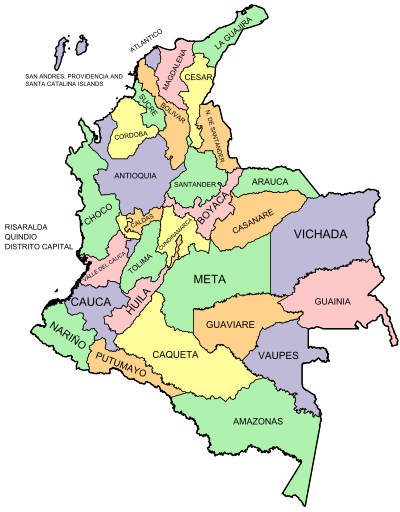
\includegraphics{departamentos.png}
\caption{Map of Departamentos in Colombia}
\end{figure}
\FloatBarrier

Capital District, Antioquia,Valle del Cauca, Cundinamarca, Atlántico and Bolivar are the six largest \textit{departamentos} in Colombia and we only consider them for the following analysis. The table below reports the results from model 2-3 in Table 2 and model 1 and 4 from Table 3 of Rueda 2016.

\FloatBarrier
\begin{table}[]
    \caption*{Extension of Tables 2 and 3 Subsetted to Only the Six Largest Departmentos}
 \singlespacing   
    \centering
{    
\scalebox{0.70}{

\begin{tabular}{l*{1}{cccc}}

\hline\hline
  \multicolumn{1}{l}{\large Dependent Variable:}&\multicolumn{2}{c}{ Vote Buying, Citizens' Reports}&\multicolumn{2}{c}{Vote Buying, Monitors' Reports}\\
                    &(1)&(2)&(3)&(4)\\
                    

\hline

Polling station size
 &-1.437&      -0.744&      -1.170&      -10.61\\
&(-3.50)&     (-1.81)&     (-1.70)&     (-1.71)\\
\hline
Municipality controls&no&yes&no&yes \\
Municipality fixed effect&&  & no&yes\\

Observations&        1317&        1308&         223&         223\\
\hline\hline
\multicolumn{2}{l}{\footnotesize \textit{t} statistics in parentheses}\\
\end{tabular}}}
\end{table}



\newpage
\section{Conclusion}
Our results suggest that, while preserving a high number of observations, the significance of many of the results which Rueda reports drops out. Rueda's variable of interest, polling place size, loses significance when controls are added for Citizens' Reports (Extension of Table 2, Column 1 with Controls Added), for all results with subsetting for National and State Elections, when dropping outliers, and when subsetting for only the largest departamentos. However, the sign of the coefficient does not change for any of these except for the second column of the national elections subset, which also exhibits a very high t statistic. Thus, it is clear that the conclusions which Rueda draws are not highly robust to extension of the analysis, or to subsetting of the data. However, the suggestion that larger polling places have less vote buying appears to be consistent, if not statistically significant.

\end{document}
